\documentclass[12pt]{article} \usepackage{times} \usepackage{graphicx}
\usepackage{cite} \usepackage[margin=1in]{geometry} \usepackage{bm}
\usepackage{cleveref} \usepackage[font=small,labelfont=bf]{caption}
\usepackage{subcaption}
\captionsetup[subfigure]{subrefformat=simple,labelformat=simple}
\renewcommand\thesubfigure{(\alph{subfigure})} \geometry{a4paper}
\usepackage{float}
%\usepackage{cite}
\newcommand{\beginsupplement}{% \setcounter{table}{0}
\renewcommand{\thetable}{S\arabic{table}}% \setcounter{figure}{0}
\renewcommand{\thefigure}{S\arabic{figure}}% } \usepackage{array}
\newcolumntype{L}[1]{>{\raggedright\let\newline\\\arraybackslash\hspace{0pt}}m{#1}}
\newcolumntype{C}[1]{>{\centering\let\newline\\\arraybackslash\hspace{0pt}}m{#1}}
\newcolumntype{R}[1]{>{\raggedleft\let\newline\\\arraybackslash\hspace{0pt}}m{#1}}

\begin{document} \title{Tunable collective behavior in active cytoskeletal
assemblies} \author{Simon L. Freedman, Shiladitya Banerjee, Glen M. Hocky,
Aaron R. Dinner} \date{} \maketitle \begin{abstract} Cells can modulate the
  mechanical properties of the actin cytoskeleton in remarkable ways to
  maintain structural integrity, move and divide. This behavior is achieved
  through crosslinking proteins and bundling agents that dynamically control
  cellular structure, as well as active motors that generate active stresses
  and regulate intracellular transport. {\em In vitro} model systems using a
  small subset of purified proteins have revealed the minimal components
  necessary to confer this wide range of mechanical behaviors. Here, we take
  the same approach using agent-based computational modeling, and investigate
  the collective dynamics of disordered cytoskeletal assemblies, consisting of
  semi-flexible filaments, dynamic crosslinkers, and molecular motors. By
  tuning the properties of individual cytoskeletal elements, such as filament
  length, crosslinker stiffness, or motor kinetics, we explore the collective
  phases of actomyosin networks across dynamic regimes inaccessible to
  experiments. Our work elucidates the diverse pathways for cytoskeletal
  contractility, polarity organization, and molecular transport, and provides
  testable predictions for future experiments on reconstituted cytoskeletal
  assemblies.  \end{abstract} \section{Introduction} The actin cytoskeleton
serves as a dynamic scaffold that allows eukaryotic cells to actively change
shape, move, and adapt to their micro-environment. Although the cellular
cytoskeleton constitutes a complex network of protein-protein interactions,
{\em in vitro} model systems have revealed the minimal set of components
required to exhibit a wide range of active mechanical behaviors including
contractility and polarity organization\cite{murrell2012,murrel2014,
takiguchi1991}. In this work, we investigate the range of collective behaviors
accessible to a minimal system consisting of cytoskeletal filaments,
crosslinking proteins, and active molecular motors. Many groups have produced
remarkable results using systems consisting only of these components, but a
necessary limitation in those studies is the difficulty to control precisely
some of the properties of constituents in the system. For example, filament
stiffness, filament length, crosslinker length, and crosslinker affinity are
all important biological parameters which vary in cells in complex and often
coupled manner. The goal of this work is to present a mathematical model, in
the form of a non-equilibrium molecular dynamics simulation, that can
efficiently explore the phase space of this actin, myosin, and crosslinker
system. This mathematical model can guide our understanding of the relationship
between the microscopic biochemical protein-protein interactions and the
macroscopic mechanical functionality of the ensemble. Additionally, because the
model simulates actin, myosin, and crosslinkers in space and time, it will
enable us to learn the trajectory of an ensemble, and how intermediate
mesoscopic structures tune network functionality.  \par Extensive research
illuminated the behavior of myosin in muscle cells, where actin filaments are
arranged in parallel bundles termed sarcomeres; a bundle of myosin heads walks
towards the barbed end of two anti-parallel actin filaments and the resulting
tension produces muscle contraction\cite{huxley1969}. However, in the
cytoskeleton of nonmuscle cells, there is no inherent ordering of actin or
myosin filaments, so while interactions between individual myosin and actin
filaments exist, how they act in concert to produce a variety of behaviors is
an active area of research \cite{murrell2012, stam2015, murrell2015}.  Recent
experimental studies \cite{murrell2012, murrell2014} have reconstituted
networks of actin and myosin, and analyzed how changing their respective
concentrations and lengths, can effect the ability of a disordered ensemble to
contract and form static structures. They have also incorporated various actin
binding proteins (crosslinkers) into their experiments such as filamin, scruin,
and $\alpha$-actinin, as these control network connectivity, and are
instrumental in crosslinking actin filaments to form long lasting, force
propagating bundles and networks \cite{gardel2004, murrell2012, murrell2014,
murrell2015}. The goal of all of these experiments is to develop a phase
diagram that shows the importance of key players of active networks, such as
myosin density \cite{murrell2012}, actin bundle rigidity \cite{murrell2012},
and cross-linker density\cite{murrell2014} in structure formation and force
generation within the cytoskeleton.  \par For example, by varying the density
of myosin added to a reconstituted actin network, one can vastly effect its
biomechanical behavior. At low motor density, the myosin will translocate large
distances but will not cause the network to contract\cite{burov2013}. Above a
critical density, the myosin will contract the network and raising the density
further will result in more extensive contraction. However, there also appears
to exist a second critical density past which more motors are ineffective at
increasing contractility \cite{murrell2014}. These \textit{in vitro}
experiments have also been used to probe the underlying mechanisms that control
the ensemble network behavior.  To date, results strongly suggest that actin
filament buckling and severing as well as relative actin and myosin sliding are
all necessary for network contraction \cite{murrell2012, murrell2014}.  \par To
probe the microscopic origin of these complex behaviors, we have developed a
simulation model, motivated both by {\em in vitro } experiments as well as
several previous computational models of actin and myosin. Some of these models
were designed to understand rheological properties of crosslinked actin
networks \cite{mackintosh1995,head2003,wilhelm2003,kim2009}, some have been
focused on the ensemble motion of motors with respect to
filaments\cite{nedelec2007,erdmann2012,stam2015}, while others have aimed at
understanding larger, structure related questions, such as how disordered
assemblies of filaments and motors collectively form asters \cite{gordon2012}
or contract \cite{wang2012,dasanyake2011,kim2014,ennomani2016}. Our model is
constructed by including many of the best features of these preceding models.
We will use the potential energy for an actin filament as described by Head et
al., for simulating actin filaments that can both bend and stretch, and also
initialize our networks similarly, by placing crosslinkers at intersections to
form well connected networks. In contrast to references \cite{head2003,
dasanyake2011}, we will simulate non-equilibrium dynamics, including
fluctuations due to non-zero temperature,  cross-linkers and myosins binding
and unbinding, and the processive activity of myosin.  We have used predictions
from \cite{stam2015} to extrapolate numerical parameters for the binding
kinetics of a myosin mini-filament as they relate to a single myosin head.
Force propagation rules and binding kinetic equations will be similar to those
of \cite{nedelec2007, gordon2012} with slight differences in how we actually
simulated the fluctuating filaments.  \par In this work, we show that this
model is well bench-marked to reproduce known experimental results for actin
filaments, ensembles of actin and crosslinkers (passive networks), and
ensembles of actin and myosin (active networks).  At the polymer level, we will
reproduce predicted spatio-temporal fluctuations of actin filaments.  For
passive crosslinked networks we will reproduce known stress strain
relationships. For active networks, we will reproduce well-understood velocity
distributions of actin filaments in a myosin motility assay. These results
demonstrate that it is possible to capture many key properties of cytoskeletal
networks within a single model which has not been optimized to reproduce any
particular set of experiments.  \par We then show that these simulations
predict non-trivial emergent dynamical behaviors which are tunable based on the
properties of the filaments, crosslinkers and motors involved. We find that
crosslinker affinity modulates filament bundling and network coarsening in a
non-monotonic manner. We show that crosslinker stiffness governs the strain
stiffening response of these networks in a simulated rheology experiment.  \par
We introduce motors into our networks and demonstrate how ensembles of randomly
oriented actin filaments and crosslinkers can be rearranged by myosin motors to
form tunable structures with distinct biophysical and mechanical functionality.
We show that motor-dependent contraction produces polarity sorted networks and
predict how that behavior depends on the concentration of motors. We use these
results to interpret emergent contractility as a competition between bundling
and polarity sorting. Finally, we study how varying the filament length, motor
density, and motor-filament binding affinity can change the way in which the
motors work in concert to translocate actin filaments, which may have
implications for how to optimize the rate at which behaviors such as polarity
sorting and contractility would be observed. 

%Using this model we successfully explore canonical F-actin experiments, such
%as the motility assay and crosslinked network rheology, and show how tuning
%the microscopic parameters of these experiments can yield a variety of
%biomechanically distinct macroscopic structures.


%The collective activity of many-particle systems where pair-wise particle
%interactions are well understood can be elucidated via molecular dynamics
%simulations. A biomolecular example involves the proteins actin and myosin in
%the cytoskeleton of non-muscle cells. In that environment, actin monomers
%polymerize into polar actin filaments (F-actin) which are microns long and
%nanometers thick, and myosin motor proteins aggregate onto $0.4\mu m$ long
%backbones to form myosin minifilaments \cite{niederman1975}. For precessive
%motors, such as myosin II, the binding of myosin to actin, followed by ATP
%hydrolysis and subsequent unbinding, results in the relative motion of myosin
%with respect to actin toward the positive (barbed) end of an actin filament.
%In the cytoskeleton, this motion drives many biological processes, including
%endocytosis, cell-division and maintenance of cell shape The mechanism through
%which myosin can walk on actin has been extensively studied in muscle cells,
%where actin filaments are arranged in parallel bundles called sarcomeres. A
%myosin filament binds to two antipolar sarcomeres, walks toward the barbed end
%of both, and the tension along the myosin pulls the sarcomeres together,
%resulting in muscle contraction\cite{huxley1969}.  However, in the
%cytoskeleton of nonmuscle cells, there is no inherent ordering of actin or
%myosin filaments, so while interactions between individual myosin and actin
%filaments exist, how they act in concert to produce a variety of behaviors is
%an active area of research \cite{murrell2012, stam2015, murrell2015}. 

\section{Results} The most striking biological function of actomyosin networks
is their contractility, which results in muscle cell contraction, and is
instrumental in motility and division in non-muscle cells.  That these complex
macroscopic mechanisms arise stochastically from simple microscopic
interactions suggests the ability to engineer materials with controllable
network topologies and dynamics.  Recently, in-vitro experiments of
reconstituted actomyosin networks have demonstrated this controllable
architecture by varying motor density and crosslinker density and showing how
they effect contractility\cite{murrell2012, murrell2014}. Our model shows a
similar dependence of contractility on motor density.  Additionally, we show
that we can tune two different macroscopic organizational techniques: bundling,
in which dynamics crosslinkers pin filaments into robust networks, and polarity
sorting, in which motors align filaments by their polarity.  \par In the
interest of computational efficiency we have chosen to coarse grain actin
filaments, and crosslinker proteins at length scales relevant for network
behavior. Actin filaments are modeled as polar worm-like chains (WLC) such that
one end of the chain represents the barbed end of a filament and the other end
represents its pointed end. Crosslinkers are modeled as Hookean springs such
that both ends of the spring (heads) can bind and unbind from filaments.
Experiments have shown that adding crosslinkers to assemblies of F-actin yields
actin bundles \cite{gardel2004, murrell2012, murrell2014} and that increasing
crosslinker density can increase the length scale of contraction
\cite{murrell2012}. Our results show that varying the stiffness of these
springs changes the rheology of an assembly of crosslinkers and filaments,
while varying the binding affinity effects the magnitude of actin bundling.
\par We parameterized our model in $2D$ similar to the nearly flat in vitro
reconstitutions of actomyosin, as this setup is sufficient to reproduce
structures of biological interest, and allows us to simulate larger systems for
longer times.  Because we use a $2D$ system to represent a $3D$ experiment, we
exclude the steric interactions of filaments and crosslinkers, to account for
some of the freedom lost from the reduction in dimensionality.
\subsection{Crosslinkers and filaments form bundled networks} The rapid binding
and unbinding of crosslinking proteins from actin filaments can reorganize
initially disordered filaments into thickly bundled networks.  This behavior is
distinct from motor-driven contractility, because the overall network structure
changes, without explicit force dipoles to strain and buckle filaments. We have
found that we can tune this bundling mechanism by changing the
crosslinker-filament binding affinity.  \par To demonstrate this behavior,
thirteen simulations were initialized with $500$ $15\mu m$ worm-like-chain
filaments scattered on a $75\mu m\times 75\mu m$ simulation cell, and $0.15\mu
m$ crosslinkers doubly bound at filament-filament intersections.  The
assemblies then evolved via Brownian dynamics for $200s$.   Each simulation had
a different dissassociation rate for crosslinkers $k_{off}^{cl}$ varying
logarithmically between $0-1800 s^{-1}$.  The results are shown in
\Cref{fig:bundle}.  \par \begin{figure}[H] \centering
  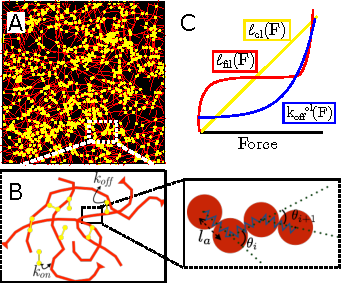
\includegraphics[scale=1.2]{figs/t0.pdf} \caption{\label{fig:t0}Initial
  configuration of actin filaments (red) for (A) assemblies which initially
  have crosslinkers (yellow, one third shown) placed at intersections and (B)
  assemblies with motors $\rho_m=0.1\mu m^{-2}$ (white) scattered throughout.
} \end{figure} The magnitude of bundling was measured by the radial
distribution function of actin filaments, $g(r) = P(r)/(2\pi r \delta r\rho)$
where $P(r)$ is the probability that two beads on different filaments are a
distance $r$, $\delta r =0.05 \mu m$ is the bin size and $\rho = 500/(75\mu
m)^2$ is the number density. As seen in \Cref{fig:bundle} C-D, the relationship
between $k_{off}^{cl}$ and $g(r)$ is non-monotonic. A disassociation rate that
is too low will not allow for significant restructuring from the initially
random configuration, and a disassociation rate that is too high will not yield
stable structures. However, at intermediate values of $k_{off}^{cl}$, a stable,
thickly bundled network can be formed.  \par \begin{figure}[H] \centering
  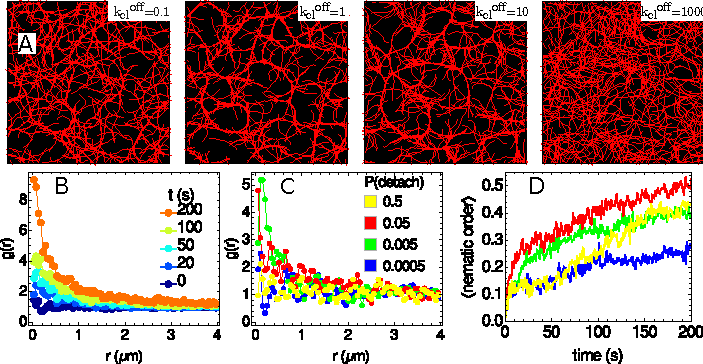
\includegraphics[scale=1.2]{figs/bundling/full_figure.pdf} \caption{%
    \label{fig:bundle}% (\textbf{A}) Actin filament (red) assemblies after
    $t=200s$ for varying disassociation constants. Filaments in red.
    (\textbf{B}) Radial distrbiution function of beads on an actin filament for
    the $k_{off}=20 s^{-1}$ at various times throughout the simulation. As the
    simulation proceeds, the higher peak at lower $r$ values shows the bundling
    increasing.  (\textbf{C}) Radial distribution function of actin filaments
    at $t=200s$ for varying $k_{cl}^{off}$.  The curves show non-monotonic
    behavior, as both high and low $k_{cl}^{off}$ have a shorter correlation
    distance than curves with mid-range $k_{cl}^{off}$.  (\textbf{C}) We
    measure this monotonicity by marking the distance at which $80\%$ of the
    area under the curves in (B) are covered. Lower values mean longer
    decorrelation lengths, indicating a larger magnitude of bundling. We also
    show that the difference in filament strain across these simulations is
    minimal, less than $0.025$, and shows no clear relationship with the radial
    distribution functions. Contrast this with contracting networks in
    \Cref{fig:contract}, where where filament strain ranges from $0$ to $0.35$
    and correlates with network divergence.  } \end{figure} \subsection{Strain
  stiffening behavior of crosslinked networks is tunable} \par The material
  properties of cross-linked F-actin networks are generally characterized using
  rheology. In a common experiment, actin and crosslinker proteins are mixed
  and form a crosslinked mesh. The mesh is placed in a rheometer and then
  sheared by a prestress $\sigma_0$. The prestressed network then undergoes a
  sinusoidal differential stress of magnitude $d\sigma<<\sigma_0$. By measuring
  the resulting strain, one can calculate the differential elastic modulus
  $G(\sigma_0) = {d\sigma\over d\gamma}$.  In experiments using a stiff
  crosslinker, such as scruin, the dependance of the differential modulus on
  high prestress is $G\propto\sigma_0^{3/2}$, indicating that this shear
  stiffening is a direct result of the nonlinear response of stretching actin
  \cite{gardel2004,lin2010}. Experiments using more compliant crosslinkers,
  such as filamin, have found a softer stiffening response, $G\propto\sigma_0$,
  indicating that a significant amount of stress is going into the
  crosslinkers, and not the actin\cite{kasza2009}.  \par These results suggest
  that the shear stiffening behavior of a crosslinked network can be tuned by
  varying the crosslinker stiffness. To test this possibility, the
  configuration of filaments shown in \Cref{fig:t0} was reproduced with varying
  crosslinker stiffness $k_{cl}$.  To inhibit network restructuring, the
  detachment rates of the crosslinkers was set to zero.  An affine strain of
  $\delta\gamma=0.001$ was applied such that the horizontal position of every
  actin bead ($x_a$) was shifted \begin{equation} x_a \rightarrow x_a +
    \delta\gamma \left( {y_a\over Y} \right) \label{eqn:sllod} \end{equation}
  following the overdamped SLLOD equations of motion \cite{evans1984}. The
  periodic boundary was simulatenously shifted following the the Lees-Edwards
  convention \cite{allen}. The mesh was then allowed to relax for $t_{relax} =
  0.001 s$ before the next strain of $\gamma$. This was performed for
  $T_f=0.5s$ so that the total strain was $\gamma T_f/t_{relax}=0.5$.
  Increasing $t_{relax}$ did not significantly change the simulation results as
  seen in \Cref{fig:tRelax10}.  \par The strain stiffening scaling for each
  crosslinker stiffness was measured by calculating $w$, the strain energy
  density at each timestep \begin{equation} w(t) = {1\over X Y}\left(\sum_f{
    U_f}+\sum_{cl}{U_{cl}}\right) \label{eqn:sed} \end{equation} where $U_f$ is
  defined in \Cref{eqn:Ufil} and $U_{cl}$ is the potential energy of each cross
  link, and averaging over windows of size $t_{relax}$ to obtain $w(\gamma)$.
  \Cref{fig:stress} shows the results of these calculations for various values
  of crosslinker $k_{cl}$. By varying the ratio of filament to crosslinker
  stiffness, we were able to vary the power law scaling of the strain energy
  density with respect to the strain. For extremely low $k_{cl}$, the sheared
  networks behaved as $w\propto \gamma$ or $G={d^2w\over d\gamma^2}=0$ as if
  the network had no resistance to shear, while for high $k_{cl}$,
  $w\rightarrow\gamma^4$. Thus, one can tune the behavior of these networks
  from being liquid-like, with $w\propto\gamma$, through the elastic solid
  regime of $w\propto\gamma^2$ as well as strain stiffening regimes of
  $w\propto\gamma^3$ and $w\propto\gamma^{3.5}$ observed in
  experiment\cite{gardel2004, kasza2009}.  \begin{figure}[H] \centering
    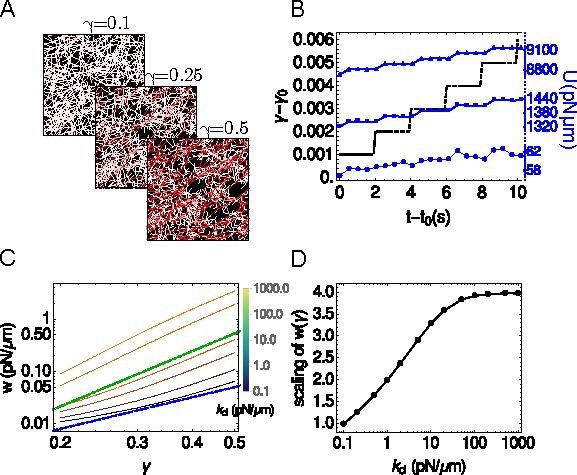
\includegraphics[scale=1.2]{figs/elasticity/shear_result.pdf} \caption{%
      \label{fig:stress}% (A) Snapshots of a strained network
      ($k_a=k_{cl}=1000$) at $t=0.1s$, $t=0.25s$ and $t=0.5s$.  Color indicates
      stretching energy on each link, with white being the lowest and red being
      the highest.  (B) The potential energy of the network as a function of
      time shown at different strains $\gamma_0=0.1$ (circles) $\gamma_0=0.25$
      (squares) and $\gamma_0=0.4$ (triangles) where $t_0=\gamma_0\times 1s$.
      Black dashed line shows the strain.   (C) Strain energy density
      ($w=U/area$) for various values of crosslinker stiffness $k_{cl}$. Blue
      dashed line indicates expected behavior for an elastic solid $w\propto
      \gamma^2$ and green dashed line indicates strain stiffening behavior of
      $w\propto \gamma^{3.5}$ as observed in \cite{gardel2004,lin2010}.  (D)
    Power law of $w$, evaluated via least squares fit to $ln(\gamma)$ vs
  $ln(w)$.  } \end{figure} \subsection{Motors sort filaments} Motors are
modeled as crosslinkers with the caveat that a head bound to a filament will
process toward the filament's barbed end (see \Cref{sec:methods_motors} for a
full description).  This implementation allows for filament sliding and
filament buckling, as seen in \Cref{fig:toys}, both of which are instrumental
for actomyosin contractility \cite{murrell2012}.  In large networks, motors can
perform these mechanisms, as well as translocate across filaments, and increase
network connectivity\cite{murrell2014}.  \begin{figure}[H] \centering
  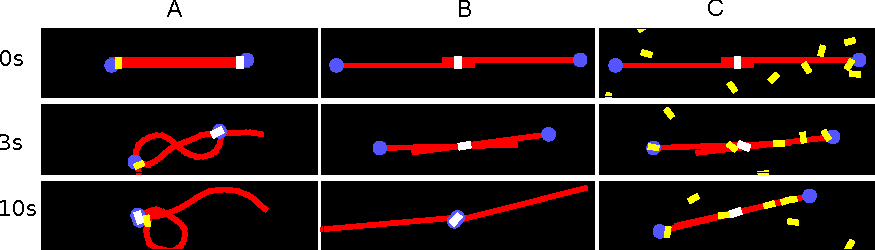
\includegraphics[width=\textwidth]{figs/minimal.pdf}
  \caption{\label{fig:slide} \label{fig:toys}% Time series of three
  antiparallel $10\mu m$ filaments (red) interacting with a minimal set of
  motors (white) and crosslinkers (blue) for $10s$. Barbed ends of filaments
  are marked by a blue dot.  (A) Filaments are semiflexible ($21$ bead-spring
  chain) and pinned on the left by a crosslinker, so the motor-filament
  interaction yields contraction via buckling.  (B) Filaments are rigid
  ($2$-bead-spring chains) and unpinned, so motor-filament interaction yields
  that filaments are slid past each other. Thus, they transition from an
  initially extended state, to a contracted state at $t=3s$ and back to an
  extended state at $t=10s$.  (C) Same as (B) but with a population of
crosslinkers near the filaments that stabilize the system in the contracted
state. } \end{figure} To isolate the role of active motors on assemblies of
semiflexible filaments, the actin assembly in \Cref{fig:t0} was generated
without  crosslinkers at filament intersections, but with $0.5\mu m$ motors
were scattered uniformly throughout the simulation cell.  In these simulations,
the motor duty ratio was kept near unity to replicate the behavior of a myosin
minifilament, while the density of motors was varied between simulations.  \par
The results, shown in \Cref{fig:polarity_sorting}, indicate that at higher
motor densities, filaments were sorted by polarity, but were not clustered.
Motors aggregated on the barbed ends of filaments and thereby brought the
barbed ends together, to form asters. The magnitude of polarity sorting was
measured by calculating the average distance of a bound motor from the barbed
end of filament to which it was bound. As seen from \Cref{fig:polarity_sorting}
A-B, increasing motor density had the effect of decreasing this distance,
indicating a larger magnitude of polarity sorting. It appears therefore that
this form of restructuring is highly tunable.  \begin{figure}[H] \centering
  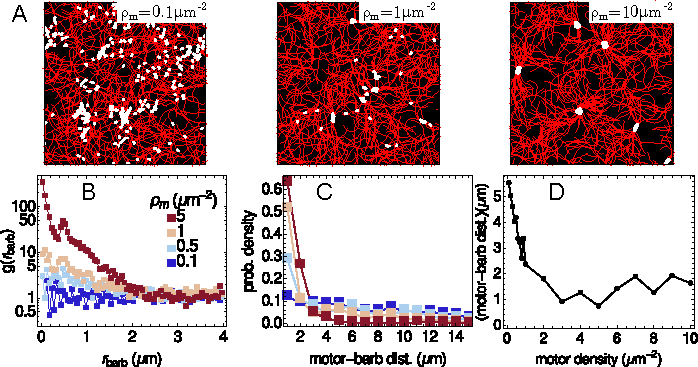
\includegraphics[scale=1.2] {figs/polarity_sorting/ps_fig.pdf} \caption{%
    \label{fig:polarity_sorting}% (A) Networks at their polarity sorted end
    configuration ($t=96s$).  Filaments in red, motors in white. A maximum of
    $1000$ motors are shown in each case.  (B) Histograms of the distance of an
    attached motor head from the barbed end of the filament to which it is
    attached for varying motor density at $t=96s$.  (C) The average distance of
    a motor head from the barbed end as a function of motor density.  (D)
    Radial distribution function for barbed ends shows a strong dependence on
    motor density. For $\rho_m=5\mu m^{-2}$, a peak is also visible at the
    motor rest length $l_m=0.5\mu m$.  } \end{figure} \subsection{Contractility
  emerges from competition between bundling and polarity sorting} \par When
  both crosslinkers and motors are combined with semiflexible filaments, the
  assemblies become contractile.  To demonstrate this behavior, actin filament
  assemblies were initialized to the configuration in \Cref{fig:t0} with
  crosslinkers at their intersections with motors scattered uniformly
  throughout the cell. The motor density varied between simulations from
  $0.1-10\mu m^{-2}$.  The crosslinkers were kept sticky with a low duty ratio,
  while the motors were highly active with a high duty ratio. This ensured that
  connectivity of the network was almost exclusively controlled by crosslinkers
  while force generation was controlled by motors.  \par The results of these
  networks can be seen in \Cref{fig:contract}. The effective contractility was
  measured by interpolating a velocity field from the displacement vectors of
  filament beads, and measuring the divergence of the velocity fields as is
  done in ref \cite{murrell2014}. A negative divergence indicates a contractile
  network. As evident in \Cref{fig:contract}(B), higher motor density leads to
  larger contractility. \Cref{fig:contract}(D) shows that actin buckling, here
  measured as the change in the end to end distance $s$ of an actin filament
  \begin{equation} s = \left(1 -
    {|r_{15}-r_0|\over\sum_{i=1}^{15}{|r_i-r_{i-1}|}}\right)
    \label{eqn:fil_strain} \end{equation} correlates with contractility,
  suggesting that the primary mechanism driving contractility in these flexible
  networks is buckling, as seen in experiment \cite{murrell2012}.
  \begin{figure}[H] \centering
    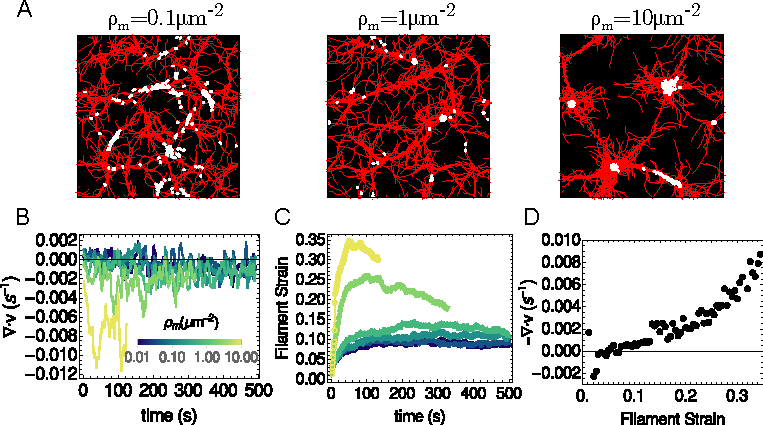
\includegraphics[scale=1.2]{figs/divergence/div_fig.pdf} \caption{%
      \label{fig:contract}% Assemblies with motors and crosslinkers yield
      contraction. (A) Networks at their largest contractility for different
      motor densities. Filaments in red, motors in white. Only $1000$ motors
      are shown in each case.  (B) Average divergence as a function of time for
      networks of varying motor density. Networks with a higher density of
      motors are more contractile.  (C) Average filament strain (defined in
      \Cref{eqn:fil_strain}) as a function of time for the same networks.  (D)
      Correlation between filament strain and network strain (measured as
      negative of divergence for all times and all motor densities, averaged
      over bins of size $0.005$ } \end{figure}  \subsection{Modulating ensemble
    motor behavior} While the force dependent detachment and speed of an
    individual myosin motor is well approximated by the input behavior
    described in \Cref{sec:methods_motors}, the ensemble behavior of many
    myosins is not input, and could provide a benchmark that the simulation is
    accurately representing active actomyosin assays \cite{walcott2012}. One
    experiment involving an ensemble of motors is the motility assay, in which
    a layer of myosin is adhered to a plate, and actin filaments are placed on
    top of the myosin. Because the myosin cannot diffuse, they instead slide
    the actin filament across the assay.  Although this experiment typically
    involves single myosin heads, and not myosin minifilaments, we believe that
    functionally the situations would be equivalent, with the substitution that
    each model motor head approximates the activity of dozens of single
    molecule myosin heads.  Various groups \cite{harris1993, umemoto1990} found
    a nonlinear dependance of the speed of an actin filament across the assay
    on the concentration of myosin, the length of the actin filament, and the
    concentration of ATP in the sample. By allowing filaments to interact with
    more motors, one can increase the filament monotonically to a critical
    speed.  \par To explore this experiment, we randomly distributed motors on
    a $(50\mu m)^2$ periodic simulation cell and constrained one head of each
    motor to remain in place. Filaments were also placed in the simulation cell
    and allowed to interact with the unconstrained motor heads. The number of
    motor-filament interactions was manipulated in three ways: by varying the
    motor concentration $\rho_m$, the filament contour length $L$, and the duty
    ratio $r_D = k_m^{on}/(k_m^{on}+k_m^{off})$.  The results are shown in
    \Cref{fig:motility}, where we have used the dimensionless parameter $\rho_m
    L^2 r_D$ to describe the various experiments.  \par In general, the
    findings were qualitatively similar to the experimental results.  For low
    motor density, filament length and duty ratio, transverse filament
    fluctuations dominate over longitudinal motion as the filament is not being
    propelled by motors faster than diffusion. However, as these variables are
    increased, longitudinal motion dominates. This can be seen from the mean
    squared displacement, plotted in \Cref{fig:motility}(D), where low $\rho
    L^2 r_D$ yields diffusive behavior with an $\langle r^2 \rangle \propto t$,
    and the motion becomes ballistic with $\langle r^2\rangle\propto t^2$ as
    $\rho L^2r_D\propto 100$.  The speed of this motion plateaus at
    $v_{||}\approx 1\mu m/s$ which is the average unloaded motor velocity, as
    seen in experiment. \Cref{fig:motility}(C) shows that aside from being
    propelled, filaments are also buckled in the presence of a large number of
    motors, as filament strain increases with increasing $\rho_m L^2 r_D$.
    Although there are no explicit crosslinkers, at a high enough
    concentration, motors near the barbed end of a filament will pin the
    filaments for a short time, and induce buckling the same way crosslinkers
    do in contractile networks.  \begin{figure}[H] \centering
      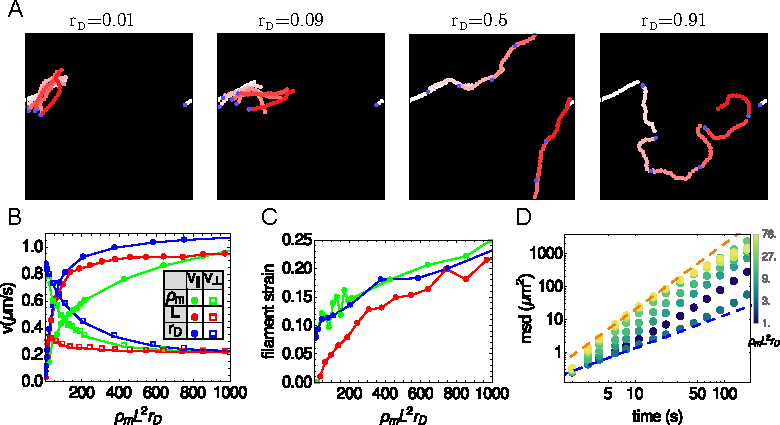
\includegraphics[scale=1.2]{figs/motility/mot_fig.pdf} \caption{%
        \label{fig:motility}% (A) Position of a filament for $\rho_m = 10\mu
        m^{-2}$ and $L = 16\mu m$ for different values of the duty ratio. White
        filament is $t=0$ and dark red is $t=90s$. Blue dot marks the barbed
        end of filaments.  (B) Longitudinal filament speed (circles)
        monotonically increases to a plateau while transverse speed (squares)
        decreases with larger motor density, filament length, and duty ratio.
        Green: $\rho$ variable, $L=15\mu m$, $r_D=0.95$; Red: $\rho_m=4\mu
        m^{-2}$, $L$ variable, $r_D=0.95$; Blue: $\rho_m = 10\mu m^{-2}$,
        $L=15\mu m$, $r_D$ variable.  (C) Filament strain, defined in
        \Cref{eqn:fil_strain}, as a function of dimensionless parameter,
        indicates that while the motor is being propelled by motors, it also is
        being buckled.  (D) Mean squared displacement for various values of
        $\rho_m L^2 r_D$ shows that the transition from diffusive (blue dashed
      line) to ballistic (red dashed line) behavior occurs at low values of
    this parameter.     } \end{figure}
%%%%%%%%%%%%%%%DISCUSSSION%%%%%%%%%%%%%%%%%%%%%
\section{Discussion} The goal of this paper is to introduce a framework that
could accurately and efficiently simulate active networks of F-actin, myosin,
and crosslinker proteins to explore the various structural phases that this
system can produce. In doing so, we have shown that our model can reproduce the
key results of canonical actomyosin experiments. When simulated networks were
sheared, strain stiffening was observed and filament speed scaling in simulated
motility assays matched experimental results. Networks with dynamic
crosslinkers were shown to form bundles, and networks with motors and
crosslinkers contracted.  We have also expanded significantly on these
experiments. 

\par For crosslinked networks, we showed that the scaling of strain stiffening
can be tuned by changing the crosslinker stiffness. Many other models have
successfully studied the viscoelastic properties of crosslinked actin networks
\cite{mackintosh1995, head2003, wilhelm2003, kim2009}.  For example, Head, et
al., used a similar simulation to ours but with straight rod filaments, and
bending potentials at rod intersections, and was able to identify three elastic
regimes, characterized by the mean distance between crosslinkers and the
temperature \cite{head2003}. Similar models used non-Hookean crosslinkers to
show how unfolding can yield strain softening at large strain
\cite{didonna2007}.  Others $3D$ models, with explicit filament bending have
examined the frequency dependence of these networks and reproduced theoretical
predictions\cite{gittes1998,kim2009,muller2014}.  Our contribution in this area
is that we have shown that by modeling crosslinkers as idealized Hookean
springs, and varying their stiffness, one can change the scaling of strain
stiffening.  This is particularly interesting, given that recent experimental
findings suggest that one can engineer actin binding proteins of varying
stiffness\cite{vieregg2016}.  

\par The ensemble motion of a many myosin motors with respect to a single actin
filament has also been studied via simulation, in order to develop a realistic
model of a myosin minifilament.  Erdmann and Schwarz, who used Monte Carlo
simulations to verify a master equation that expresses the probability that $N$
motors are bound at time $t$ to a single filament\cite{erdmann2012} were able
to make accurate predictions for the duty ratio and force velocity curves for
myosin minifilaments.  Stam et al. used simulations to study force buildup on a
single filament by a multi-headed motor and found distinct timescale regimes
over which different biological motors could exert force and act as
crosslinkers \cite{stam2015}. These models of actin-myosin interaction are
important to understand the mechanics at the level of a single filament, and
their results can be incorporated into larger network simulations.  However,
our results show that even a minimal model of actin and myosin is able to
capture the ballistic, longitudinally processive behavior of actin filaments in
a motility assay seen in experiments. 

\par Other actomyosin models have explored the driving mechanisms behind
contractility.  Dasanyake, et. al., extended the model in \cite{head2003} to
include a term in the potential energy that corresponded to myosin motor
activity, and observed the emergence of force chains that transmit stress
throughout the network\cite{dasanyake2011}.  Wang and Wolynes \cite{wang2012}
model the F-actin networks as a graph of crosslinkers (nodes) and rigid actin
filaments (edges) in which myosin motor activity is simulated via antisymmetric
kicks along the filaments and predict a binary phase diagram of networks which
are either contractile or not as a function of cross linker and myosin
densities. While the simplicity of these models is intriguing, they do not
account for explicit filament buckling, and their integration is performed via
Monte Carlo, more applicable to structure formation than dynamics.  We have
shown that using an agent based model we can reproduce the experimentally
observed contractility of actomyosin networks, that it scales with motor
density, and that it correlates with filament buckling, both of which have been
confirmed in in vitro reconstitutions \cite{murrell2012,murrell2014}.

\par Contractility and structure formation has also been explored in the
context of agent based models.  Nedelec used dynamic simulations of ensembles
of filaments and motor proteins to explore aster formation in
microtubule-kinesin assemblies, as well as motility and contractility in
actomyosin \cite{nedelec2002,nedelec2007,ennomani2016}.  Kim used an agent
based approach of filaments, motors and crosslinkers, to explore a variety of
topics, including bundling in crosslinked networks and force generation by
myosin motors\cite{kim2009b, kim2014}.  While the bundling observed in
\cite{kim2009b} was the result of crosslinkers that explicitly bind parallel
filaments, we have that generic crosslinking leads to network coarsening and
that this bundling effect depends strongly, and non-monotonically on the
crosslinker-filament affinity. These bundled networks have the important
physical property of being able to transmit forces large distances, and are
thought to serve the biomechanical functionality of forming force chains to
propagate stress throughout the cell. 

\par Additionally, we showed that we can tune polarity sorting in filament
assemblies.  Polarity sorted networks can be used to by load-carrying motors to
transmit cellular goods large distances, so insight into how a cell modulates
this behavior could be extremely helpful in biophysics and active matter. While
this polarity sorting is similar to the aster formation seen in
\cite{nedelec2002,gordon2012}, we have shown that the process will also occur
when filaments are semiflexible, have developed a reliable order parameter for
measuring this process, and shown that the magnitude of this parameter
increases monotonically with motor density. 

\par While our model is thorough in what it aims to simulate it is limited by a
few experimental observations that are currently not implemented. First, the
structure of myosin minifilaments is significantly more complex than a two
headed spring. As mentioned, these minifilaments have dozens of heads, which
allows them to walk along multiple filaments and could result in subdiffusive
behavior \cite{scholz2016} and significantly increase local network elasticity
\cite{murrellTalk}.  Another limitation of our system is that the actin
filaments are static, and will not polymerize, depolymerize or sever. Within
actomyosin assays it is clear that recycling of actin monomers and to a lesser
degree, filament severing plays an important role in
contraction\cite{murrell2012}. Within the cytoskeleton, actin treadmilling is
also important for shape production. Additionally, these simulations are all
run in $2D$ and without steric interactions, and dimensionality and volume
exclusion may play important roles.  While we intend to address and investigate
these limitations in future works, we believe that the successful benchmarking
of the simulation at various levels is a significant argument in favor of the
current setup.

\par There are still many unanswered questions regarding cytoskeletal
actomyosin networks that we hope to addressed using this simulation, such as
how they controllably reshape the cell membrane, and they form force
propogating chains across the cytoskeleton.  In particular, it is significantly
easier to measure local forces and energies in simulation than in experiment,
so we expect this model will aid the process of isolating the particular
mechanisms involved in restructuring these polymer assemblies. We stress,
however, that the applicability of such a simulation package reaches beyond
studying the phases of actomyosin networks.  We believe this simulation can
shed light on a variety of active polymer assemblies.  \par Similar networks
that involve other proteins also exist in the cytoskeleton, such as
microtubule-kinesin-dynein networks and could be investigated using this
simulation methodology.  Furthermore, the cytoskeleton demonstrates how
populations of simple machines can self assemble into active materials with
useful mechanical properties, and one can use this simulation to efficiently
design these types of self assembled materials. Thus, the non-equilibrium
molecular dynamics framework of this simulation can be used to model and study
many open questions in active matter and biophysics.

\section{Methods}  \subsection{Actin Filaments} Actin filaments are treated as
a worm-like chain, with each filament represented as a set of $N+1$ beads
connected by $N$ harmonic springs (links), with an additional harmonic angular
potential applied on the $N-1$ angles along the chain, as depicted in
\Cref{fig:filament}(A). The linear springs penalize stretching of individual
subunits and the $N-1$ angular harmonic springs penalize bending and enforce
the length scale over which the filaments are semi-flexible. 

The internal forces on actin filaments can be obtained from the gradient of the
potential energy $U_f$ \begin{eqnarray} U_f &=& U_{stretch} + U_{bend}\\
  U_{stretch}&=&{k_a\over2}\sum_{i=1}^{N}{(|d_i| - l_a)^2}\\\nonumber
  U_{bend}&=&{\kappa_B\over 2l_a}\sum_{i=2}^N{\theta_i^2}\\\nonumber
  \label{eqn:Ufil} \end{eqnarray} where $d_i = r_i-r_{i-1}$, $\theta_i =
\arccos{\left({d_i\cdot d_{i-1}\over |d_i||d_{i-1}|}\right)}$, $k_a$ is the
stretching force constant, $\kappa_B$ is the bending modulus, and $l_a$ is the
equilibrium length of a link.  \par For a confined semiflexible filament, it
has been show that for a polymer of a given persistence length $L_p$, the
shortest length that should be considered as unbending ($l_a$) is given by
$l_a\approx A^{2/3}L_p^{1/3}$ where $A$ is a length scale associated with the
confinement of the filament \cite{odijk1983}. In these simulations, filaments
were confined by nearby motors and crosslinkers. Since the smallest motor or
crosslinker density used was $\rho_m=0.1\mu m^{-2}$, $A\ge1/\sqrt{0.1\mu
  m^{-2}}\Rightarrow l_a\ge5\mu m$. In general, we used $l_a=1\mu m$.  The
  bending force constant is derived from the persistence length $L_p$ such that
  $\kappa_B = L_p k_B T$ where $k_B$ is Boltzmann's constant and $T$ is the
  temperature \cite{rubinstein}. Experimentally, the stretching force constant
  has been measured to be in the approximate range $k_a=40-70pN/nm$
  \cite{kojima1994, higuchi1995}; however, simulating a network of filaments
  with this large of a stiffness is computationally inefficient since the
  maximum timestep of a simulation is inversely proportional to the largest
  stiffness in the simulation. Therefore, we chose ${\kappa_B\over l_a} <<k_a$,
  so that the filaments were still much easier to bend than to stretch,
  enabling us to run simulations of experimentally relevant dimension. We show
  that our simple filament model exhibits expected behavior for a semiflexible
  filament in the next section and we have further verified that $k_a$ did not
  effect the persistence length of the filament, as seen in
  \Cref{fig:wlc_supp}.  \par Since actin bending is instrumental for actomyosin
  contraction, and simulating precise bending moduli is non-trivial, we tested
  our filaments by measuring spatial and temporal fluctuations and comparing
  with theoretical predictions.  In a two dimensional WLC, a bending of two
  adjacent segments is expected to result in a local change in free energy of
  ${\kappa_B\over2l_a\theta_i^2}$, and it is predicted that \cite{frontali1979}
  \begin{equation} \langle\theta^2(l)\rangle = {l\over L_p} \label{eqn:thsq}
  \end{equation} \begin{equation} \langle\cos(\theta(l))\rangle =
    \exp{(-l/2L_p)} \label{eqn:costh} \end{equation} where $\theta(l) =
  \theta_j - \theta_i$ where $1<i<j\le N$, $l = l_a(j-i)$ and $L_p$ is the
  persistence length. To test our model against these equations, we simulate
  $100$ filaments of $L=200\mu m$ and $\kappa_B=0.08 pN\mu m^2$ at $T=300K$ for
  $T_f = 100s$ and measured the resulting filament configuration every $1s$. We
  discard the first $10$ seconds of each simulation to allow equilibration, and
  we used only the middle $150 \mu m$ of the filament to calculate these
  correlation functions.
%For each of the $90000$ filament configurations, and for each
%$l\in{0,1,2,..,150}\mu m$, $\theta^2(l)$ and $\cos(\theta(l))$ were
%calculated, and their respective averages are plotted in \Cref{fig:avgTh},
%along with the expected behavior given the input $\kappa_B$.  
\Cref{fig:kb} shows that the measured persistence length, obtained by
performing a least squares fit to plots of $\log{(\langle cos(\theta(l))\rangle
)} $ for various values of $\kappa_B$ yields the expected result over at least
$3$ orders of magnitude. Further measurements of the persistence length as well
as verifications of its independence on other filament parameters is available
in the supplement \Cref{lpCalc}.  \par An additional prediction for
semiflexible filaments is the scaling of fluctuations with time.  Fluctuations
transverse to the filament orientation have been shown to increase as a
function of time as $\langle dr_{\perp}^2\rangle\propto t^{3/4}$ while
longitudinal fluctuations have been shown to follow the power law $\langle
dr_{||}^2\rangle\propto t^{7/8}$ \cite{everaers1999}. To tests these
predictions, we followed the procedure outlined in \cite{everaers1999} and
generated $N = 100$ initial filament configurations of a $20\mu m$ filament.
For each configuration we ran $M = 100$ simulations of the filament fluctuating
for $1s$. At each time step we collected the $2N$ positions of the filament
ends, $r_e(t)$. We then calculated the eigenvalues of the covariance matrix
$cov(r_e(t)\cdot \hat{i},r_e(t)\cdot \hat{j})$ where $i,j\in\{x,y\}$.  The
larger eigenvalue $\lambda_1(t)$ corresponds to the slower longitudinal
fluctuations (i.e., $\lambda_1(t)\propto t^{7/8}$) while the smaller eigenvalue
corresponded to the faster perpendicular fluctuations ($\lambda_2(t)\propto
t^{3/4}$). We show  in \Cref{fig:filament}(C) that the our simulation exhibits
scaling of these eigenvalues in good agreement with the prediction of Ref.
\cite{everaers1999}.  \begin{figure}[H] \centering
  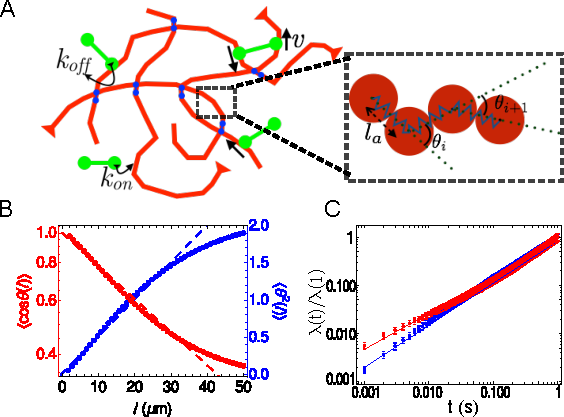
\includegraphics[scale=1]{figs/filament/pl_fig.pdf}
  \caption{\label{fig:filament} (A) Sketch of semiflexible filaments (red);
  motors (green) binding, unbinding, and walking; and crosslinkers (blue)
  connecting filament intersections. Zoom in of the filament model shows a
  segment of the bead spring chain, identifying the angle used in
  \Cref{eqn:Ufil}.  (B) Decorrelation of tangent vectors (red dots) and
  fluctuations in angles between links (blue dots) as a function of the arc
  length between them. Red dashed line is $e^{-s/2L_p}$ shows the expected
  behavior from the input bending modulus of $0.08 pN-\mu m^2$ and blue dashed
  line has slope $1/L_p$.  (C) Eigenvalues of covariance matrices for the
  positions of endpoints of filaments as a function of time. We analyze
  fluctuations of $N=100$ filaments, with each point the average over the $2N$
  eigenvalues for $\lambda_1(t)$ and $\lambda_2(t)$ and error bars showing the
  standard deviations for the distribution of these values. Blue dots shows the
  longitudinal fluctuations and the red dots shows the transverse fluctuations.
  Red dashed line is $t^{3/4}$ and blue dashed line is $t^{7/8}$ as predicted
  by \cite{everaers1999}.  } \end{figure} \subsection{Crosslinkers} Crosslinker
proteins dynamically connect actin filaments, thereby propogating force from
one to another. Thus model crosslinkers, must be able to attach and detach from
actin filaments, and be compliant in order to propagate force. They are
therefore modeled as hookean springs, with stiffness $k_{cl}$ and rest length
$l_{cl}$. Like actin filaments, the Young's modulus of most crosslinkers is
significantly higher than would be reasonable to simulate; therefore we set
$k_{cl} = 1-100pN/\mu m$ was so that the bending mode of actin filaments was
signicantly softer than the stretching mode of crosslinkers. Their rest length
$l_{cl}$ differs by the type of cross-linker and ranges from $~10 nm$ for
fascin to $150 nm$ for filamin.  \par At each time step of the simulation an
unattached crosslinker head is allowed to attach to nearby filaments and an
attached crosslinker head can detach.  The probability of a head attaching to
an actin filament is a Gaussian distributed random variable, such that
\begin{equation} P_{cl}^{on} = k_{cl}^{on}dt\exp(-r^2/R^2) \label{eqn:cl_on}
\end{equation} where $r$ is the shortest distance from the head to the actin
filament and $R = \sqrt{2k_B T\over k_{cl}}$ where $k_B$ is Boltzmann's
constant and $T$ is the temperature.  For crosslinker detachment we assume that
the behavior is that of a slip bond, such that a higher tensile force along the
crosslinker backbone will result in a higher probability of detachment. Thus,
\begin{equation} P_{cl}^{off} = k_{cl}^{off} dt\exp{\left(  F x_{cl}/k_B
T\right)}  \label{eqn:cl_off} \end{equation} where $F$ is the force along the
crosslinker backbone, and $x_{cl}$ is a characteristic bond length
\cite{stam2015}.  \par When a crosslinker is bound to a filaments at both ends,
it will necessarily be stretched or compressed.  If it were allowed to relax
independently of the actin filaments to which it is bound.  it would no longer
lie on those filaments. Therefore, the tensile force stored on a stretched or
compressed crosslinker is propagated onto those actin filaments via the lever
rule outlined in \cite{nedelec2002, gordon2012}. Thus, if the tensile force of
a motor at point $r_j$ between filament beads $i$ and $i+1$ is $F_{cl}$, then,
\begin{eqnarray} F_i &=& F_{cl}\left|\left( {r_j - r_i \over r_{i+1} - r_i
}\right)\right|\\\nonumber F_{i+1} &=& F-F_i \label{eqn:lever} \end{eqnarray}
will be the forces on beads $i$ and $i+1$ respectively due to the crosslinker.
\subsection{Motors}\label{sec:methods_motors} Within the cytoskeleton, tens of
myosin II motors aggregate into bipolar ensembles called myosin minifilaments
\cite{stam2015}. While the mechanochemical process through which individual
myosin motors walk along actin filaments is complex, motility assay experiments
have shown that on average bound myosin II heads walk at an unloaded speed of
$v_0\approx1\mu m/s$ along actin filaments\cite{finer1994}. To a first
approximation, minifilaments therefore should also have a mean speed of $1\mu
m/s$ (although see \cite{stam2015} and \cite{walcott2012} for higher order
measurements).  Since myosin also functions to increase the local elasticity of
networks wherever it is bound, the myosin is modeled similarly to a
crosslinker, in that it behaves like a hookean spring with two heads, a
stiffness $k_{m}$ and a rest length $l_m$. It should be noted, however, that
the two heads of this spring do not correspond directly to individual molecular
myosin heads; rather each of them represents tens of myosin molecules, and
their rate constants will reflect that notion.  It would be undesirable for a
myosin minifilament to stretch, since experimentally they have a very high
Young's modulus and it is unlikely that their length would change noticably in
the cytoskeleton. Thus we set $k_m\gg\kappa_B/l_a$ so that the bending of actin
is still the softest mode.  The rest length was set to the average length of
minifilaments \cite{niederman1975}.  Attachment and detachment kinetics for
motors are the same as for crosslinkers, subscripted with $m$ instead of $cl$
in \Cref{eqn:cl_on,eqn:cl_off}. One extra parameter is needed $k_m^{end}$ for
the detachment of myosin from the barbed end of a filament, as detachment from
the end is significantly more probable than from the rest of the filament.
Similarly, force propogation onto minifilaments is done using the lever rule
described in \Cref{eqn:lever}.  \par Unlike crosslinkers, motors process
towards the barbed end of actin filaments to which they are bound at speeds
that vary depending on the tensile force along the crosslinker.  The
relationship between motor velocity and tensile force is modeled linearly, such
that the motor head will speed up if the minifilament is compressed
(pre-powerstroke) and slow down if the minifilament is stretched (post
powerstroke) going to $0$ when the force on the minifilament is the stall force
$F_s\approx 3.85pN$ \cite{nedelec2002, gordon2012}; i.e.,  \begin{equation}
  v(F_{||}) = v_0\left( 1-{F_{||}\over F_s}) \right) \label{eqn:myo_vel}
\end{equation} where $F_{||}$ is the force on the motor, projected along the
tangent vector of the actin filaments.  The minor differences between
crosslinkers and motors allow us treat them equivalently, by setting $v_0 = 0$
for the crosslinkers.  

\subsection{Dynamics} We Langevin dynamics to solve for the motion of actin
filaments, myosin minifilaments and crosslinkers.  The Langevin equations of
motion for a spherical bead of mass $m$ and radius $R$ at position $r(t)$ at
time $t$ can be written, \begin{equation} m\ddot{r}(t) = F(t) + B(t) - 4\pi
  R\nu \dot{r}(t) \label{eqn:lang} \end{equation} where $F(t)$ is the force on
the particle due to its interactions and $B(t)$ is Brownian forcing term, to
simulate a temperature, $\nu$ is the dynamic viscosity of the bead's
environment, and we have used the Einstein relation for the damping term.
Since the fastest motion in this simulation is that of the myosin, and a
$0.4\mu m$ myosin minifilament moving at a speed of $1\mu m/s$ in a liquid at
least as viscous as water ($\nu_D=10^6\mu m^2/s$ dynamic viscosity) has a very
low Reynold's number ($Re \approx 4*10^{-7}$) we can treat the dynamics in the
overdamped limit where the equation of motion is \Cref{eqn:lang} without the
acceleration term, i.e. with $m=0$.  Furthermore, in the limit of small $\Delta
t$, we may write $\dot{r(t)} \approx {r(t+\Delta t)-r(t)\over \Delta t}$. These
two approximations allow us to rewrite \Cref{eqn:lang} as \begin{equation}
  r(t+\Delta t) = r(t) + F(t)\mu \Delta t + B(t) \mu \Delta t
  \label{eqn:overdamped} \end{equation} where $\mu = (4\pi R\nu)^{-1}$. For the
Brownian term, we use the form of Leimkuhler and Matthews
\cite{leimkuhler2012,leimkuhler2013} that has been shown to minimize deviations
from canonical averages in harmonic systems, \begin{equation}
  B(t)=\sqrt{2k_BT\over\mu \Delta t}\left({W(t)+W(t-\Delta t)\over2}\right)
  \label{eqn:baoab_brownian} \end{equation} where $W(t)$ is a Wiener process,
in this case a random number drawn from the normal distribution with mean zero
and standard deviation of unity.

\subsection{Environment} \par Because the probability of motor attachment
decays as a Gaussian function of distance from the filament, it would be highly
inefficient to attempt motor attachments with every filament in the simulation.
Rather, we choose to test for connections only within a cutoff distance
$r_c>3R/2$ (where $R$ is defined above as in \Cref{eqn:cl_on}). A grid of
lattice size $2r_c$ is drawn in the $2D$ plane of the simulation, and the
position of a filament is approximated as the points on the grid nearest to the
beads of the filament. Thus, to determine if a motor will bind to a filament at
time $t$, it is sufficient to only attempt attachment to filaments that are
indexed at the four nearest grid points to a motor.  \par In general, we use
periodic boundary conditions so as to limit effects of a boundary and to mimic
a system larger than the one we simulate. Lees-Edwards boundaries \cite{allen}
were used for shearing simulations, and hard wall boundaries have also been
implemented.  The value for $\Delta t$ in \Cref{eqn:overdamped} generally
depends on both the unloaded myosin speed $v_0$ and the largest stiffness in
the simulation $k_f$. For $k_f = 10pN/\mu m$ and $v_0=1\mu m/s$ a value of
$\Delta t = 0.00001 s$ was sufficiently low to solve \Cref{eqn:overdamped} for
hundreds of seconds without spuriously generating configurations of very large
energy.  The length and width of the simulations were chosen so as to be high
enough to avoid boundary artifacts.  A complete list of simulation parameters
used throughout this article is provided in \Cref{tab:params}.  \begin{table}
  \caption{Parameter Values} \centering
  \begin{tabular}{|C{1cm}|L{6cm}|C{2cm}|C{2cm}|C{2cm}|C{2cm}|} \hline\hline
    Symbol & Description (units) [ref] & $L_p$ & Shear & Motility Assay &
    Networks\\ \hline &\bf{Actin Filaments}& & & &\\ \hline $N_B$ & Number of
    beads & $21-201$ & $16$ & $16$ &$16$\\ $l_a$ & Link Rest Length ($\mu
    m$)\cite{odijk1983}& $1$ & $1$ &$1$& $1$\\ $k_a$ & Stretching Force
    Constant ($pN/\mu m$) & $0.01-10$ & $10$ & $1$ & $1$\\ $\kappa_B$ & Bending
    Modulus ($pN\mu m^2$)\cite{ott1993} & $0.002-5 $ & $0.08$ & $0.08$ &
    $0.08$\\ \hline &\bf{Myosin Minifilaments}& & \\ \hline $l_m$ & Rest Length
    ($\mu m$)\cite{niederman1975} & n/a & n/a & 0.5 & 0.5\\ $k_m$ & Stiffness
    ($pN/\mu m$)& n/a & n/a & $1$ & $1$\\ $k^{on}_m$ & Attachment rate at
    distance $r=0$ ($s^{-1}$)& n/a & n/a &$2-4000$ &$3600$\\ $k^{off}_m$ &
    Unloaded head detachment rate ($s^{-1}$)& n/a & n/a & $200$ &$200$\\
    $k^{end}_m$ & Unloaded head detachment rate at the barbed end of the
    filament ($s^{-1}$)& n/a & n/a &$2000$ &$2000$\\ $x_m$ & characteristic
    bond length ($\mu m$) \cite{stam2015}& n/a & n/a & $0.0004$& $0.0004$\\
    $v_0$ & Unloaded speed ($\mu m/s$) \cite{kron1986}&  n/a & n/a & $1$ &
    $1$\\ $F_s$ & Stall force of myosin ($pN$)\cite{veigel2003}& n/a & n/a &
    $3.85$ & $3.85$\\ \hline &\bf{Crosslinkers} & & \\ \hline $l_{cl}$& Rest
    Length (Filamin) ($\mu m$)\cite{ferrer2008} & n/a &$0.150$ &n/a&$0.150$ \\
    $k_{cl}$ & Stiffness ($pN/\mu m$)& n/a & $1,10$ & n/a& $1$\\ $k^{on}_{cl}$
    & Attachment rate at distance $r=0$ ($s^{-1}$)& n/a & $10^6,10^5$ &n/a
    &$3600$\\ $k^{off}_{cl}$ & Unloaded head detachment rate ($s^{-1}$)& n/a &
    0 & n/a&$0.2$\\ $x_{cl}$& characteristic bond length ($\mu m$) & n/a &
    $0.0004$ & $0.0004$ & $0.0004$ \\ \hline &\bf{Environment} & & \\ \hline
    $dt$ & Dynamics timestep (s) & $10^{-4}$ & $10^{-6},10^{-5}$
    &$2.5\times10^{-4}$ &$2.5\times10^{-4}$ \\ $T_F$& total simulated time (s)
    & $100$ & $0.5$ & $100$ & $500$ \\ $X$, $Y$ & Length and width of assay
    ($\mu m$)& n/a & $75$ & $50$ & $75$\\ $r_c$ & Mesh (actomyosin binding
    site) size ($\mu m$) & $n/a$ & $0.2 $ & $0.2 $& $0.2 $ \\ $T$ & $k_B$ *
    Temperature ($pN\mu m$)& $0.004$ & $0.004$& $0.004$& $0.004$\\ $\nu$ &
    Dynamic viscosity ($mg/(\mu m s)$) & $0.001$& $0.001$& $0.001$& $0.001$\\
    $\gamma$ & Strain (\%) \cite{stricker2010}& n/a& $0.001$&n/a&n/a\\
    $t_{relax}$ & Amount of time between sequential strains (s)& n/a& $0.001$
    &n/a&n/a\\ \hline \end{tabular} \label{tab:params} \end{table}



\section{Acknowledgements}  We thank M. Gardel, J. Weare, C. Matthews, F.
Nedelec, F. Mackintosh, and M. Murrell for helpful conversations. This research
was supported in part by the University of Chicago Materials Research Science
and Engineering Center (NSF Grant No. 1420709). S.L.F. was supported by the
Department of Defense (DoD) through the National Defense Science \& Engineering
Graduate Fellowship (NDSEG) Program. G.M.H. was supported by an NIH Ruth L.
Kirschstein NRSA award (1F32GM113415-01).  \bibliography{actosim}
\bibliographystyle{unsrt}

\beginsupplement \section{Supplement} \subsection{Algorithm Pseudocode} In
pseudocode we can describe each timestep of the simulation as follows
\begin{verbatim} For Each Bead on Each Filament: Update force from filament
stretching Update force from filament bending\end{verbatim} \verb|    Update
position via | \Cref{eqn:overdamped}\begin{verbatim} For Each Head on each
Motor (cross-linker) If head is unattached try to attach Add up forces
(stretching)\end{verbatim} \verb|    Update position via |
\Cref{eqn:overdamped}\begin{verbatim} If head is attached\end{verbatim} \verb|
Update position via | \Cref{eqn:overdamped}\begin{verbatim} Try to detach If
not detached Step toward barbed end Update attached actin with stretch force
Update neighbor lists \end{verbatim} \subsection{ Further tests of the WLC
model }\label{lpCalc} From \Cref{eqn:costh} the distribution of the square of
end to end distances can be calculated as \begin{equation} \langle
  r^2\rangle=\int_0^L{ds'}\int_0^L{ds \exp{(|s-s'|)/(2L_p)}}=4L_p L\left(
  1-{2L_p\over L}\left( 1-\exp{(-L/2L_p)} \right) \right) \label{eqn:r2}
\end{equation} Thus, \Cref{eqn:r2} provides a third method for measuring the
persistence length by averaging the observable $r_N-r_0$.  \Cref{fig:R2} shows
the results of the end to end distributions for each of these sets of
simulations for each each $L$.  We fit this data to \Cref{eqn:r2} to obtain a
third estimate for $L_p$.  See \Cref{lpCalc} for further detail regarding the
calculation of data points, error bars, and fits in these plots.  The agreement
between the three fits in \Cref{fig:filament}(B) and \Cref{fig:R2}, and the
fact that all measurements produced data in reasonable correspondance with the
input persistence length, $L_p = \kappa_B/k_BT = 20\mu m$ show that the model
correctly simulates a semiflexible filament.  In \Cref{fig:filament}(B), for
each value of $L$, the results of the $10$ simulations were averaged to give
one number $\overline{\theta^2_L(l)}$, and a standard deviation
$\sigma(\theta^2_L(l))$. These values were then averaged to obtain a single
value of $\overline{\theta^2(l)} =
\sigma(\theta^2(l))^2\sum_L{\overline{\theta^2_L(l)}\over\sigma(\theta^2_L(l))^2}$
where $\sigma(\theta^2(l))^2 = 1/\sum_L{\sigma(\theta^2_L(l))^{-2}}$. The
values for the $\overline{\theta^2(l)}$ were fit to a line via least squares
and $L_p$ was calculated as the inverse of the slope. The same process was done
for the data points in the blue curve, wherein $ln(\overline{(cos(\theta(l)})$
was fit to a line via least squares and $L_p = -1/2m$ where $m$ is the slope of
the fit line. For \Cref{fig:R2}, the data point itself is the average of
$<r^2(L)>$ over the $10$ simulations, and the error bars show one standard
deviation of the ensemble. The data is then fit to the nonlinear function in
\Cref{eqn:r2} using the \textit{Wolfram Mathematica} function
\textit{NonlinearModelFit} and a value for $L_p$ is predicted. 

\subsubsection{Further tests of the WLC model} To verify that the persistence
length was independent of the stretching stiffness $k_f$, we evaluated $L_p$
using a fit to \Cref{eqn:costh} for various values of $k_a$ as shown in
\Cref{fig:kl}. For $k_a>5pN/\mu m$ we find that $L_p$ is independent of $k_a$.
\begin{figure}[H] \begin{subfigure}{0.4\textwidth} \centering
    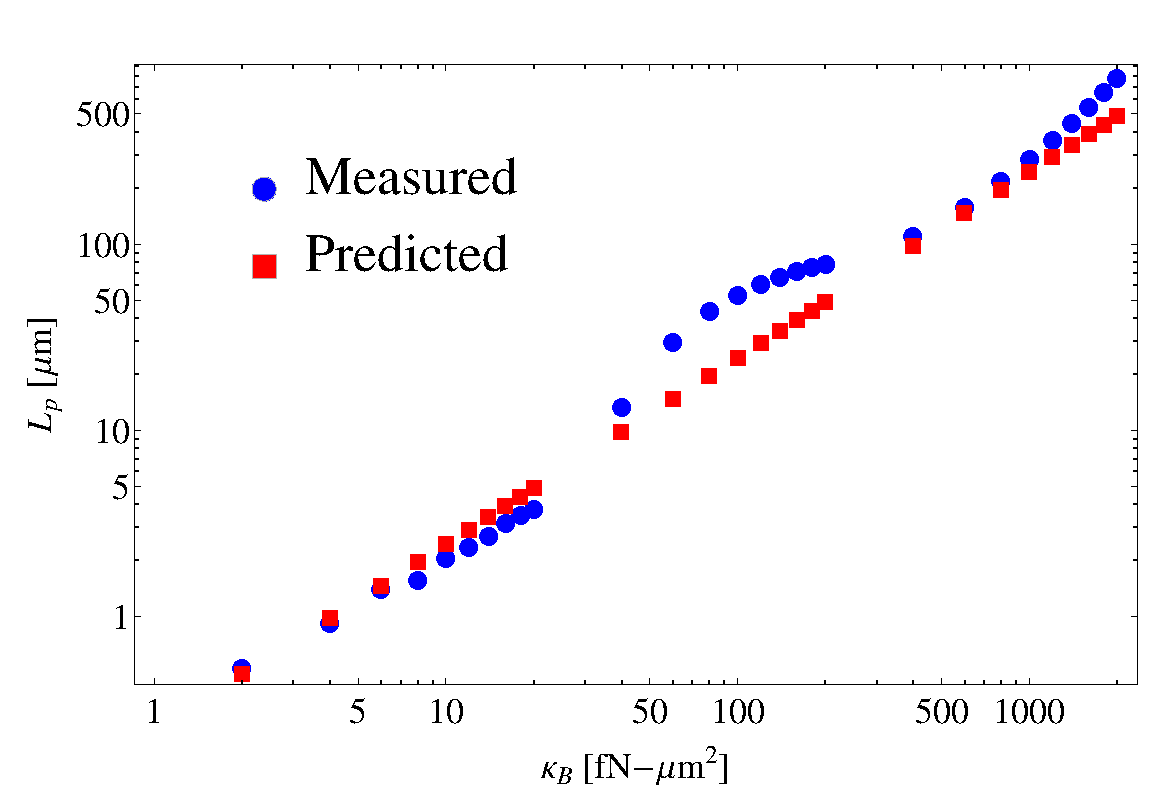
\includegraphics[width=\textwidth]{figs/filament/kb_vs_lp_fit_all.eps}
    \caption{\label{fig:kb}} \end{subfigure} ~ \begin{subfigure}{0.4\textwidth}
    \centering
    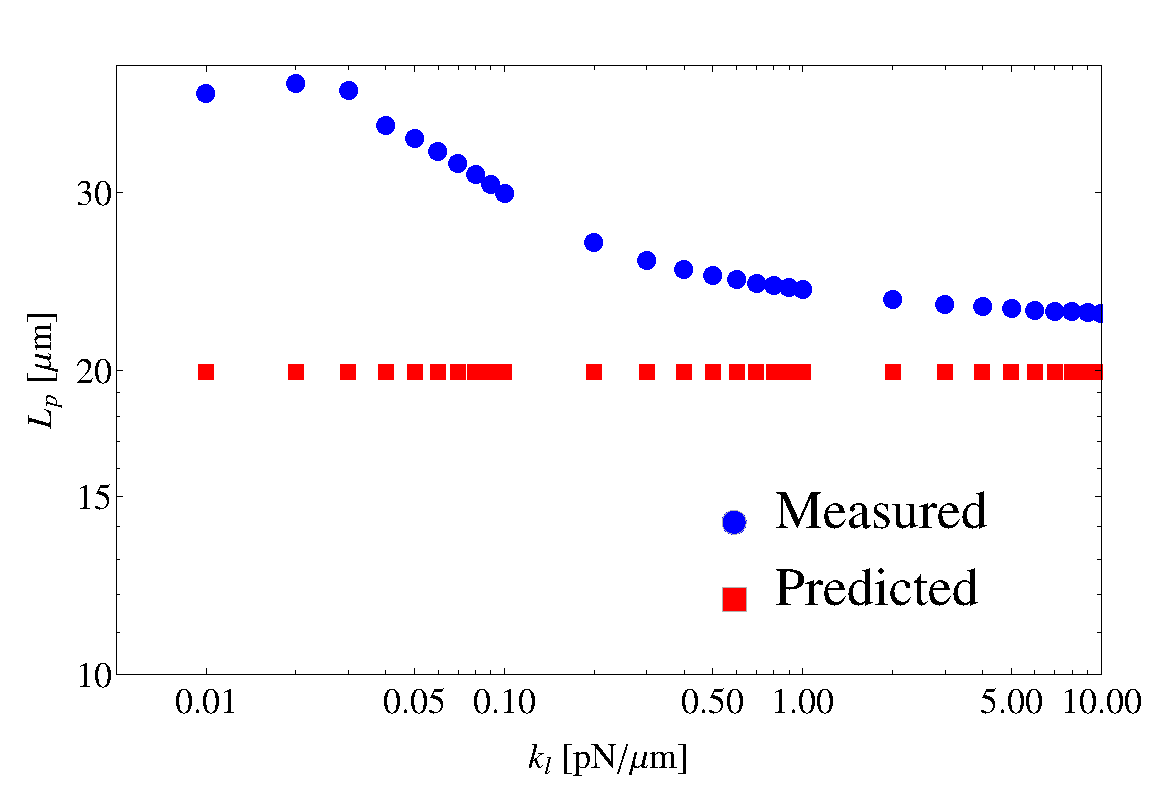
\includegraphics[width=\textwidth]{figs/filament/kl_vs_lp_fit30.eps}
    \caption{\label{fig:kl}} \end{subfigure}% ~
  \begin{subfigure}{0.6\textwidth} \centering
    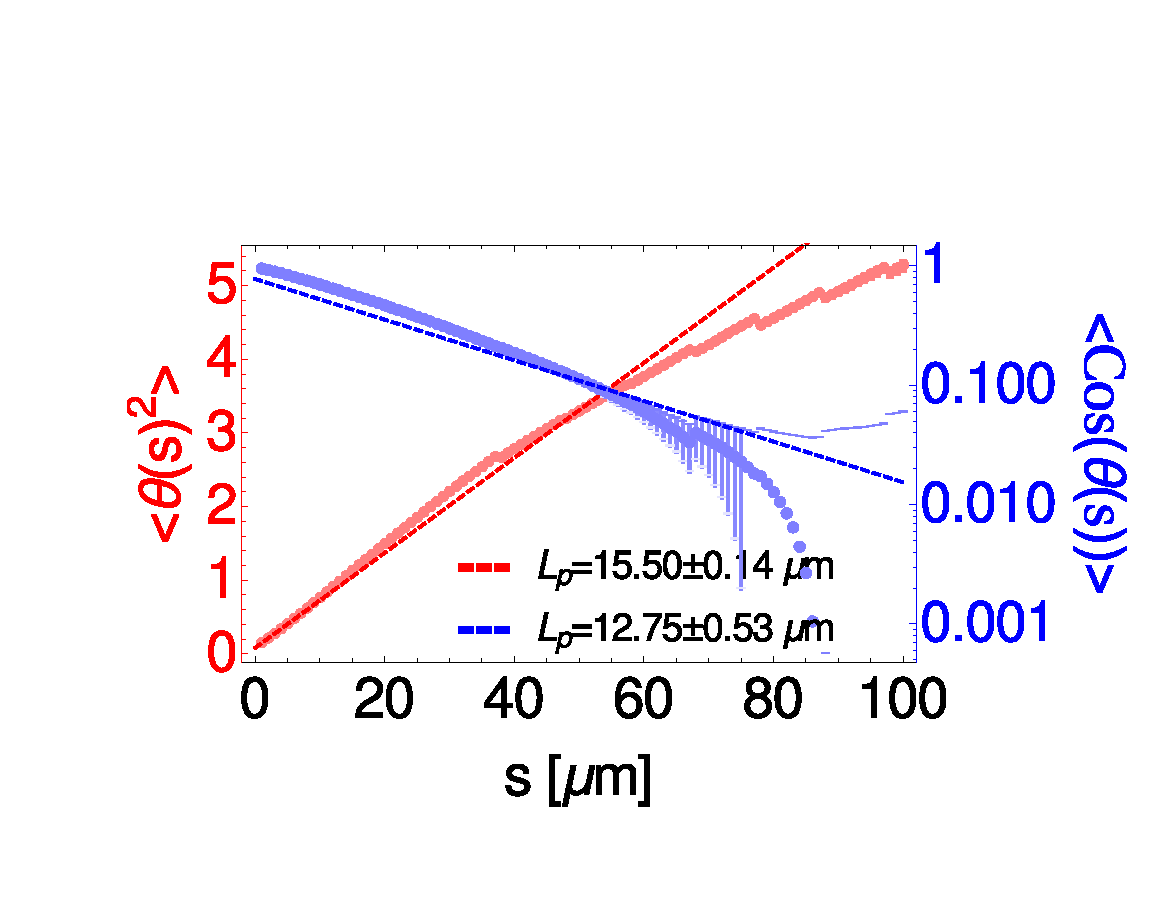
\includegraphics[width=\textwidth]{figs/filament/sAvgd_L1-100.eps}
    \caption{\label{fig:lp_vs_l}} \end{subfigure} ~
  \begin{subfigure}{0.4\textwidth} \centering
    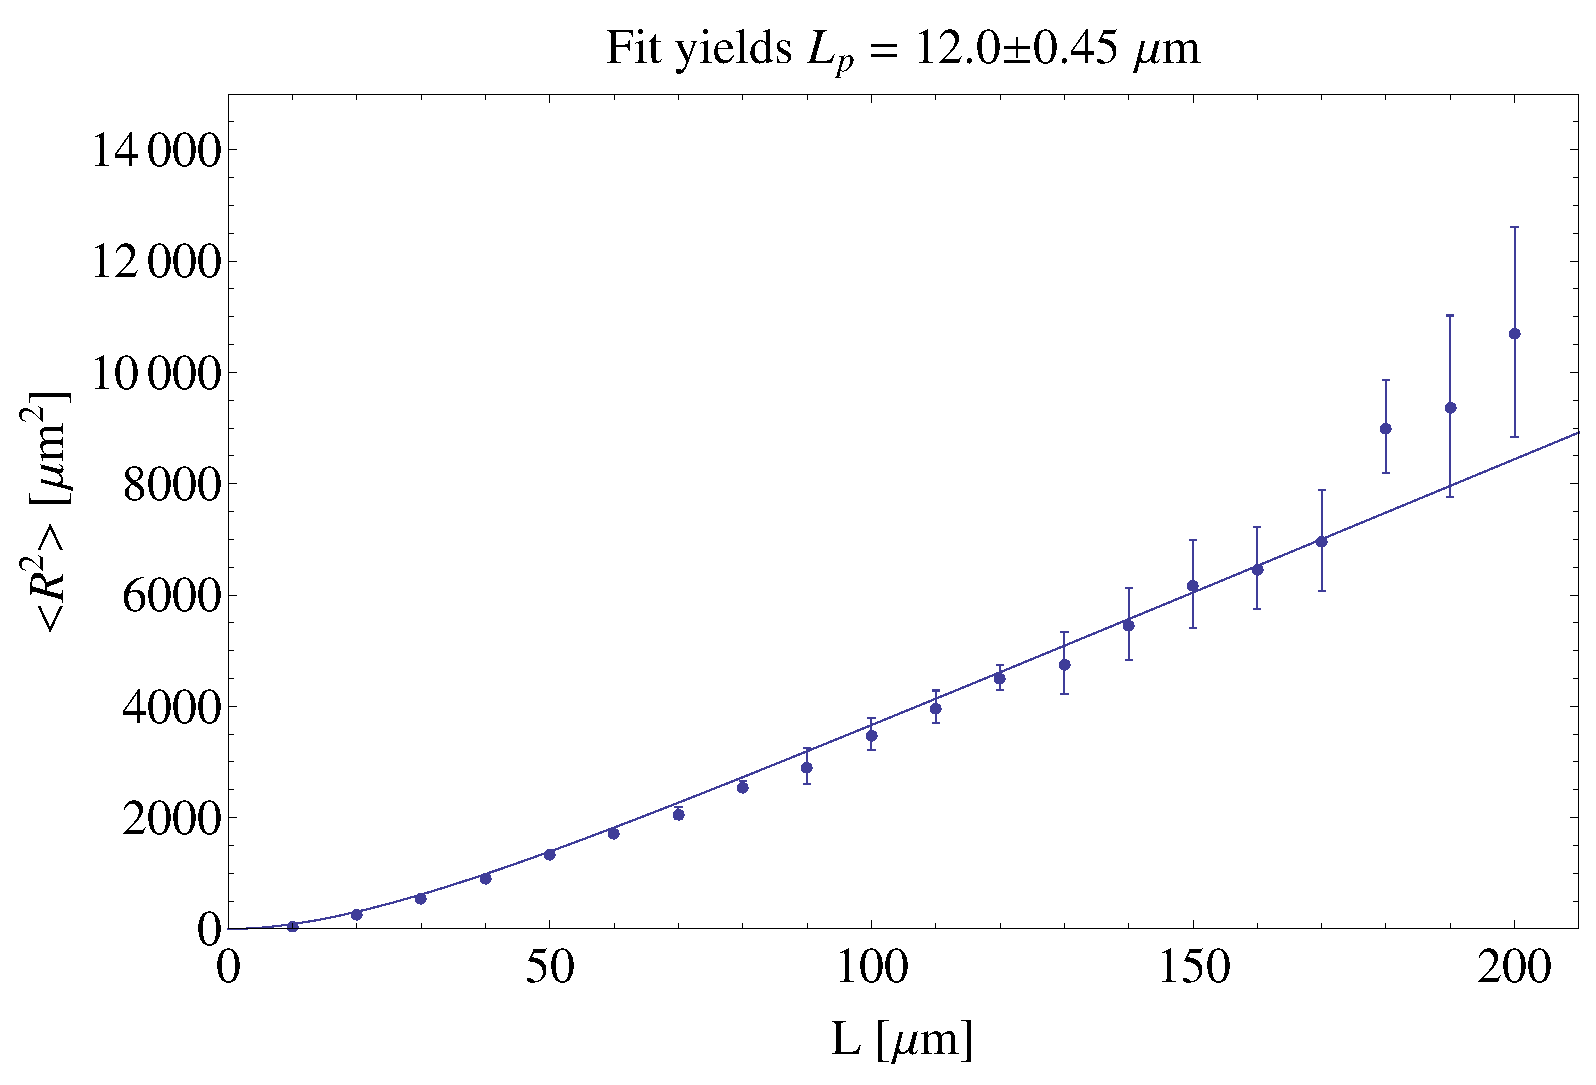
\includegraphics[width=\textwidth]{figs/filament/R2vsL.eps}
    \caption{\label{fig:R2}} \end{subfigure} \label{fig:wlc_supp} \caption{
    \subref{fig:kb} Input bending modulus vs measured persistence length over
    three orders of magnitude. Persistence length was measured by fitting a
    line to $\ln{(\langle \cos{(\theta)}\rangle)}$ in each case.
    \subref{fig:kl}Persistence length as function of stretching stiffness
    approaches correct answer for high enough stiffness.
    \subref{fig:lp_vs_l}Methods $1$ and $2$ of measuring persistence length,
    described in main text using different length filaments.  \subref{fig:R2} A
    third method for measuring persistence length, as function of end to end
    distance, described above.  } \end{figure} \subsection{Strain Stiffening}
  \label{strain_supp} \begin{figure}[H] \begin{subfigure}{0.35\textwidth}
      \centering
      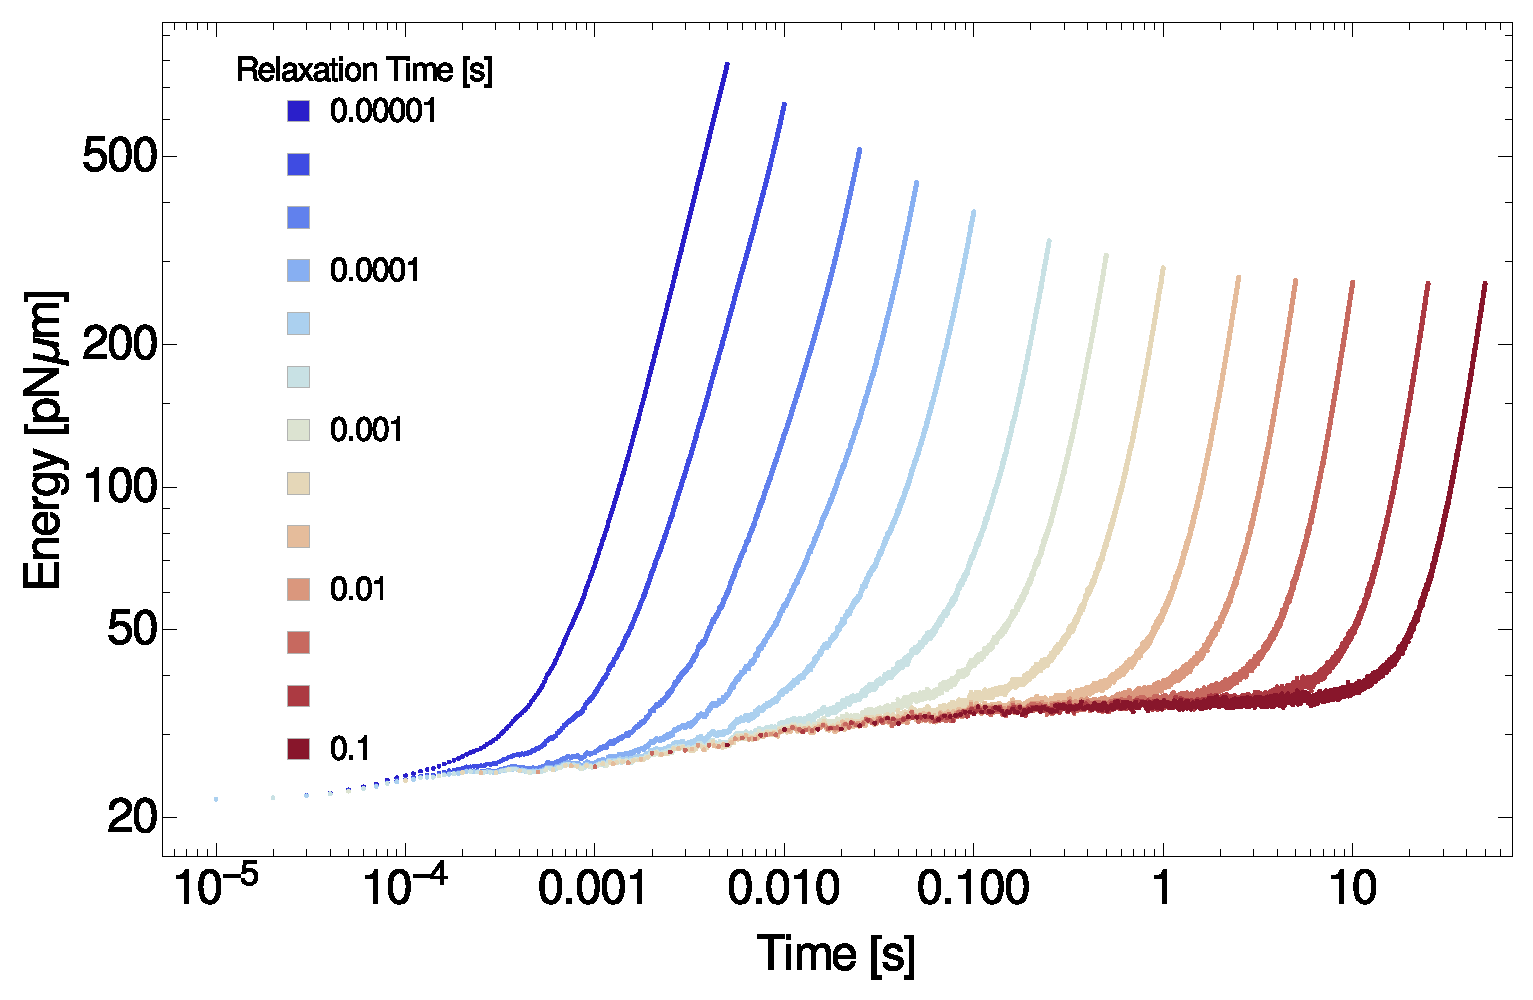
\includegraphics[width=\textwidth]{figs/elasticity/eng_vs_t_k10.eps}
      \caption{\label{fig:tRelax10}} \end{subfigure}
    \begin{subfigure}{0.35\textwidth} \centering
      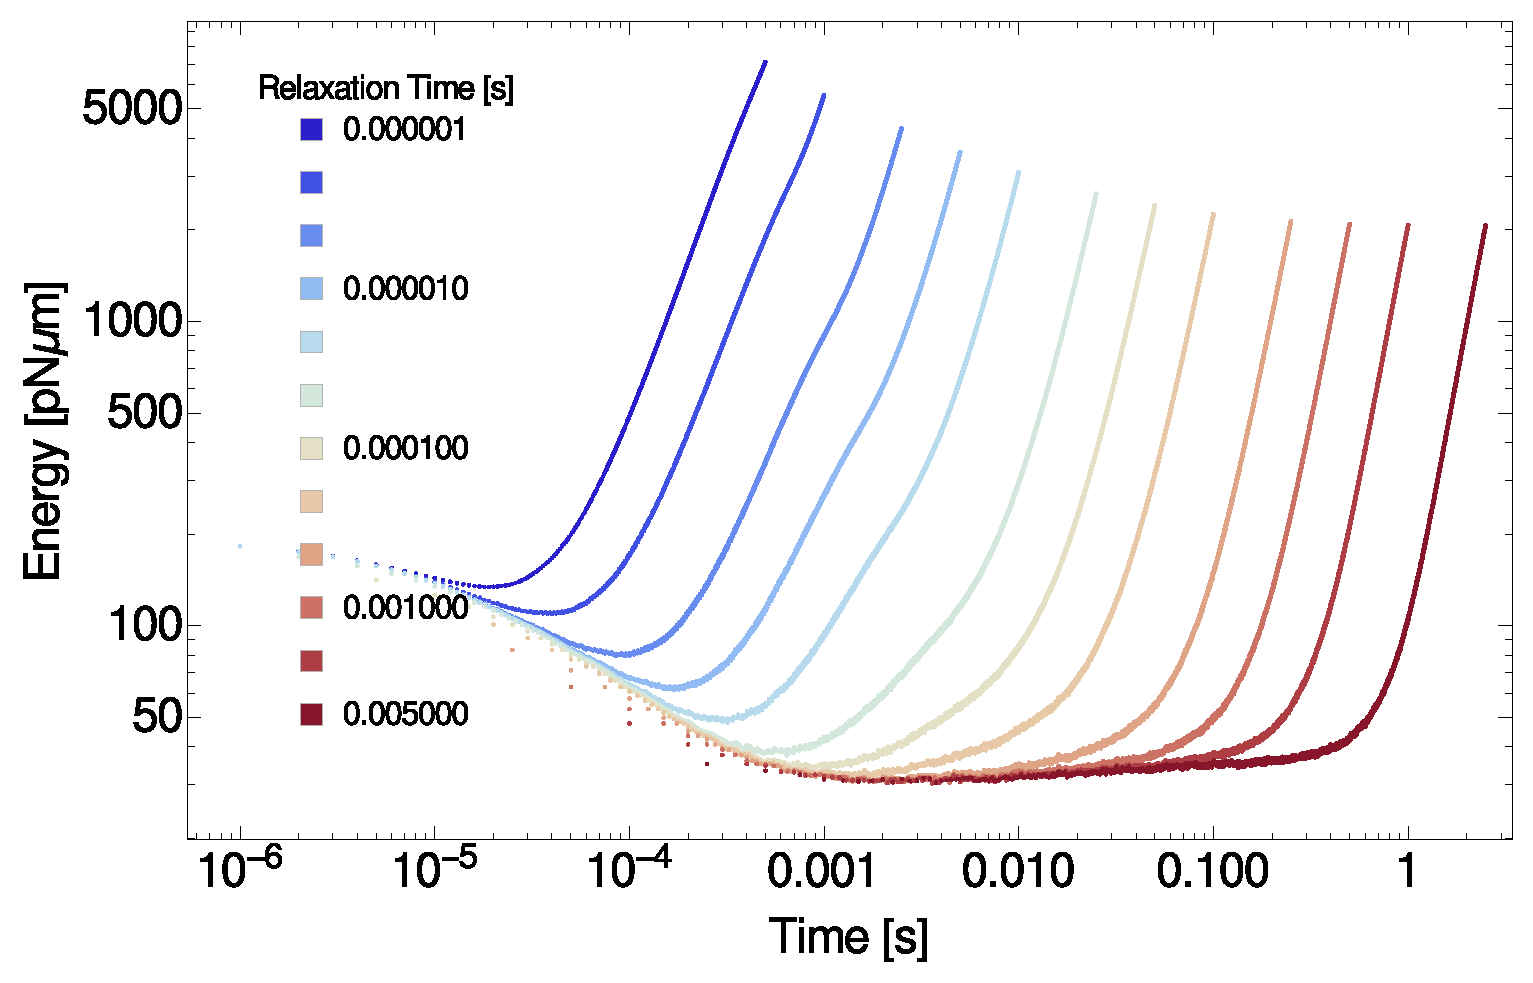
\includegraphics[width=\textwidth]{figs/elasticity/eng_vs_t_k100.eps}
      \caption{\label{fig:tRelax100}} \end{subfigure} \label{fig:tRelax}
    \caption{Strain energy as function of time for various relax times
      $t_{relax}$ for networks with \subref{fig:tRelax10} $k_{cl}=10pN/\mu m$
      and\subref{fig:tRelax100} $k_{cl}=100pN/\mu m$  crosslinked networks}.
    \end{figure} \subsection{Bundling} To contrast between bundling,
    contractility, and polarity sorting we computed the divergence of bundled
    networks, as well as the radial distribution function of the filament
    barbed ends in bundled networks. The results are shown in figure
    \Cref{fig:bundling_supp}.  \begin{figure}[H] \centering
      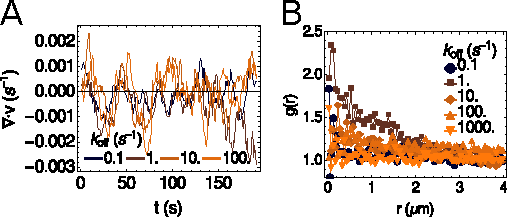
\includegraphics[width=\textwidth]{figs/bundling/bundling_supplement.pdf}
      \caption{\label{fig:bundling_supp} (A) Assemblies without motors that
      bundle do not show an average negative divergence, unlike assemblies with
      motors (\Cref{fig:contract}).  (B) The radial distribution function for
      bundled networks for the barbed end of filaments is significantly less
      peaked than for all points on the filaments (\Cref{fig:bundle}). Thus,
      the network is not polarity sorted.  } \end{figure} \end{document}
